\documentclass[12pt,fullpage,letterpaper]{article}

\newenvironment{proof}{\noindent{\bf Proof:}}{\qed\bigskip}

\newtheorem{theorem}{Theorem}
\newtheorem{corollary}{Corollary}
\newtheorem{lemma}{Lemma} 
\newtheorem{claim}{Claim}
\newtheorem{fact}{Fact}
\newtheorem{definition}{Definition}
\newtheorem{assumption}{Assumption}
\newtheorem{observation}{Observation}
\newtheorem{example}{Example}
\newcommand{\qed}{\rule{5pt}{7pt}}

\newcommand{\assignment}[4]{
\thispagestyle{plain} 
\newpage
\setcounter{page}{1}
\noindent
\begin{center}
\framebox{ \vbox{ \hbox to 7in
{\bf CS466: Introduction to Bioinformatics \hfill #1}
\vspace{4mm}
\hbox to 6.28in
{\hspace{2.5in}\large\mbox{Problem Set #2}}
\vspace{4mm}
\hbox to 6.28in
{{\it Handed out: #3 \hfill Due: #4}}
}}
\end{center}
}


\newcommand{\handout}[3]{
\thispagestyle{plain} 
\newpage
\setcounter{page}{1}
\noindent
\begin{center}
\framebox{ \vbox{ \hbox to 6.28in
{\bf CS466: Introduction to Bioinformatics \hfill #1}
\vspace{4mm}
\hbox to 6.28in
{\hspace{2.5in}\large\mbox{#2}}
\vspace{4mm}
\hbox to 6.28in
{{\it Handed Out: #3 \hfill Name (NetID): \rule[-2pt]{4cm}{0.1pt} }}
}}
\end{center}
}


\newcommand{\assgsoln}[4]{
\thispagestyle{plain} 
\newpage
\setcounter{page}{1}
\noindent
\begin{center}
\framebox{ \vbox{ \hbox to 6.28in
{\bf CCS466: Introduction to Bioinformatics n \hfill #1}
\vspace{4mm}
\hbox to 6.28in
{\hspace{2.5in}\large\mbox{Problem Set #2 Solutions}}
\vspace{4mm}
\hbox to 6.28in
{{\it Handed Out: #3 \hfill Handed In: #4}}
}}
\end{center}
}


\newenvironment{algorithm}
{\begin{center}
\begin{tabular}{|l|}
\hline
\begin{minipage}{1in}
\begin{tabbing}
\quad\=\qquad\=\qquad\=\qquad\=\qquad\=\qquad\=\qquad\=\kill}
{\end{tabbing}
\end{minipage} \\
\hline
\end{tabular}
\end{center}}

\def\Comment#1{\textsf{\textsl{$\langle\!\langle$#1\/$\rangle\!\rangle$}}}




\oddsidemargin 0in
\evensidemargin 0in
\textwidth 6.5in
\topmargin -0.5in
\textheight 9.0in

\usepackage{hyperref}
\usepackage{float}
\usepackage{pdfpages}
\usepackage{textcomp}
\usepackage{mathtools}
\usepackage{algorithm}
\usepackage{array}
\usepackage{tabu}
\usepackage{changepage}
\usepackage{amsmath}
\usepackage{amssymb}
\usepackage{lscape}
\usepackage{tikz}
\usetikzlibrary{trees}

\usepackage[noend]{algpseudocode}
\usepackage{graphicx,url,epstopdf}
\usepackage{xcolor}
\makeatletter
\def\BState{\State\hskip-\ALG@thistlm}
\makeatother
\sloppy
\usepackage{colortbl}




\newcommand\tab[1][1cm]{\hspace*{#1}}

\begin{document}

\assignment{Name: Payal Mantri\hspace{5cm}}{1}{September 7, 2022}{September 15, 2022 (11:59pm, CT)}
% Fill in the above, for example, as follows:
% \solution{Joe Smith}{\today}{1}{Fall 2012}

\pagestyle{myheadings}  % Leave this command alone

\noindent\emph{Instructions:} This homework assignment consists of five questions worth a total of 50 points. 
In addition, there is a bonus question on the third page worth an additional 6 points.
These questions are based on the material covered in Lectures 1 to 5.
\textbf{Do not forget to write your name at the top!}

\begin{enumerate}

\item[1.] \textbf{Asymptotic Running Time} [5 points]
\\
\\
Consider the following running time functions, where $n > 0$. % (the  Big-Oh notation of O() is implicit),
\begin{center}
\begin{tabular}{ c c c c c c c c c c c c } 
 %\hline
 $n^{2}$ & $n^{3}$ & $\sqrt{n}$ & $n^{2}\log(n)$ & $n\log(n)$ & $n!$ & $2^{n}$ & $n$\\
 $n(n+1) - n^2$ & $n+n^{2}$ & $n\log(n^2)$ & $n^{3}-n^{2}$ & $1$ & $n^{2}-n$ & $n^n$  & 10,000,000\\ 
 %\hline
\end{tabular}
\end{center}
\begin{enumerate}


\item[a.] Identify groups of functions such that for any pair $(f(n),g(n))$ of functions in the same group it holds that both $f(n) = O(g(n))$ and $g(n)=O(f(n))$. Note that some groups will contain a single function. [3~points]

\emph{Hint:} For example, $f(n) = 3n$ and $g(n)=n$ would be in the same group, as $f(n) = 3n = O(n) = O(g(n))$ and $g(n) = n = O(3n) = O(f(n))$.

\fbox{\parbox{\linewidth}{
\begin{itemize}
    \item $ g_{1} $(x) = \{1 , 10000000\}
    \item $g_{2}$(x) = \{$\sqrt{n}$\}
    \item $g_{3}$(x) = \{$n$ , $n(n+1) - n^2$ \}
    \item $g_{4}$(x) = \{$n\log(n)$ , $n\log(n^2)$ \}
    \item $g_{5}$(x) = \{$n^{2}$  , $n+n^{2}$ , $n^{2}-n$  \}
    \item $g_{6}$(x) = \{$n^{2}\log(n)$   \}
    \item $g_{7}$(x) = \{$n^{3}$ ,  $n^{3}-n^{2}$ \}
    \item $g_{8}$(x) = \{ $2^{n}$  \}
        \item $g_{9}$(x) = \{$n!$  \}
    \item $g_{10}$(x) = \{$n^n$  \}

\end{itemize}

}}
.\vspace{1em}
\item[b.] Arrange the resulting Big Oh running time groups in order from fastest to slowest. [2~points]

\fbox{\parbox{\linewidth}{
$ g_{1} $ , $ g_{2} $, $ g_{3} $, $ g_{4} $, $ g_{5} $, $ g_{6} $ , $ g_{7} $,
$ g_{8} $, $ g_{9} $, $ g_{10} $
.\vspace{3em}
}}
\end{enumerate}

\clearpage

\item[2.] \textbf{Sequence Alignment} [20 points]
\\
 
Consider two DNA sequences $\mathbf{v} = \mathrm{TAGATA}$ and $\mathbf{w} = \mathrm{GTAGGCTTAAGGTTA}$. 
In this exercise, we will align the two sequences using a score of +1 for a match, -1 for a mismatch, and -1 for a insertion/deletion (i.e.\ a gap penalty of 1).
We will use three different alignment algorithms. In each case, follow the specific instructions to provide requested information about the dynamic programming table or optimal alignment.  



\begin{enumerate}
\item[a.] Consider the following global alignment of $\mathbf{v}$ with $\mathbf{w}$. 
\begin{center}
\begin{tabular}{ c | c c c c c c c c c c c c c c c } 
$\mathbf{v}$ & - & T & A & G	&-&	-&	- &	- &	A & -	&-&	- &	T &	- &	A  \\
$\mathbf{w}$ & G & T & A & G & G & C & T & T & A & A &	G &	G &	T &	T &	A\\
\end{tabular}
\end{center}

Give the score for this global alignment and fill out the dynamic programming table with the corresponding backtrace (i.e. highlight the corresponding path through this table and fill in cells on path with alignment scores).  [5 points]

\vspace{.5cm}

\fbox{\parbox{\linewidth}{
\vspace{.5cm}
\begin{tabular}{|c|c|c|c|c|c|c|c|c|c|c|c|c|c|c|c|c|}
\hline
  & - &G  &T  &A  &G  & G & C & T & T & A & A  & G  & G  & T  & T  & A\\ \hline
- &\cellcolor{red!25}0  &\cellcolor{red!25}-1 &-2 &-3 &-4 &-5 &-6 &-7 &-8 &-9 &-10 &-11 &-12 &-13 &-14 &-15 \\ \hline
T &-1 &-1 &\cellcolor{red!25}0  &-1 &-2 &-3 &-4 &-5 &-6 &-7 &-8  &-9  &-10 &-11 &-12 &-13 \\ \hline
A &-2 &-2 &-1 &\cellcolor{red!25}1  &0  &-1 &-2 &-3 &-4 &-5 &-6  &-7  &-8  &-9  &-10 &-11\\ \hline
G &-3 &-1 &-2 &0  &\cellcolor{red!25}2  &\cellcolor{red!25}1  &\cellcolor{red!25}0  &\cellcolor{red!25}-1 &\cellcolor{red!25}-2 &-3 &-4  &-5  &-6  &-7  &-8  &-9\\ \hline
A &-4 &-2 &-2 &-1 &1  &1  &0  &-1 &-2 &\cellcolor{red!25}-1 &\cellcolor{red!25}-2  &\cellcolor{red!25}-3  &\cellcolor{red!25}-4  &-5  &-6  &-7 \\ \hline
T &-5 &-3 &-1 &-2 &0  &0  &0  &1  &0  &-1 &-2  &-3  &-4  &\cellcolor{red!25}-3  &\cellcolor{red!25}-4  &-5 \\ \hline
A &-6 &-4 &-2 &-2 &-1 &-1 &-1 &0  &2  &1  &0   &-1  &-2  &-3   &-4  &\cellcolor{red!25}-3  \\ \hline
\end{tabular}



\vspace{.5cm}

Alignment score:  \underline{ \quad   -3    \quad \quad   } 
}}

\clearpage
\item[b.] Consider the following fitting alignment (grayed out entries are not part of the alignment). That is, an alignment of $\mathbf{v}$ and a substring of $\mathbf{w}$ with maximum global alignment score.  

\begin{center}
\begin{tabular}{ c | c c c c c c c c c c c c c c c } 
$\mathbf{v}$  & \textcolor{gray}{-} & \textcolor{gray}{-}& \textcolor{gray}{-} &\textcolor{gray}{-} & \textcolor{gray}{-} & \textcolor{gray}{-} &	\textcolor{gray}{-} &	\textcolor{red}{T} &	\textcolor{red}{A} & \textcolor{red}{-}	& \textcolor{red}{G}&	\textcolor{red}{A} &	\textcolor{red}{T} &	\textcolor{red}{-} &	\textcolor{red}{A}  \\
$\mathbf{w}$ & \textcolor{gray}{G} & \textcolor{gray}{T} & \textcolor{gray}{A} & \textcolor{gray}{G} & \textcolor{gray}{G} & \textcolor{gray}{C} & \textcolor{gray}{T} & \textcolor{red}{T} & \textcolor{red}{A} & \textcolor{red}{A} &	\textcolor{red}{G} &	\textcolor{red}{G} &	\textcolor{red}{T} &	\textcolor{red}{T} &	\textcolor{red}{A}\\
\end{tabular}
\end{center}

Give the score for this fitting alignment and fill out the dynamic programming table with the corresponding backtrace (i.e. highlight the corresponding path through this table and fill in cells on path with alignment scores). [5 points]

\vspace{.5cm}

\fbox{\parbox{\linewidth}{

\vspace{.5cm}
\begin{center}
\hspace{-.3cm}
\begin{tabular}{|c|c|c|c|c|c|c|c|c|c|c|c|c|c|c|c|c|}
\hline
  & - &G  &T  &A  &G  & G & C & T & T & A & A  & G  & G  & T  & T  & A\\ \hline
- &0  &0  &0  &0  &0  &0  &0  &\cellcolor{red!25}0  &0  &0  &0   &0   &0   &0   &0   &0 \\ \hline
T &-1 &-1 &1  &0  &-1 &-1 &-1 &1  &\cellcolor{red!25}1  &0  &-1  &-1  &-1  &1  &1   &0 \\ \hline
A &-2 &-2 &0  &2  &1  &0  &-1 &0  &0  &\cellcolor{red!25}2  &\cellcolor{red!25}1   &0   &-1  &0  &0  &2\\ \hline
G &-3 &-1 &-1 &1  &3  &2  &1  &0  &-1 &1  &1   &\cellcolor{red!25}2   &1   &0  &-1  &1\\ \hline
A &-4 &-2 &-2 &0  &2  &2  &1  &0  &-1 &0  &2   &1   &\cellcolor{red!25}1  &0   &-1  &0 \\ \hline
T &-5 &-3 &-1 &-1 &1  &1  &1  &2  &1  &0  &2   &1   &0  &\cellcolor{red!25}2   &\cellcolor{red!25}1  &0 \\ \hline
A &-6 &-4 &-2 &0  &0  &0  &0  &1  &1  &2  &1   &0   &0  &1   &1  &\cellcolor{red!25}2  \\ \hline
\end{tabular}
\end{center}
\vspace{.5cm}

Alignment score:  \underline{ \quad   2    \quad \quad   } 
}}

\clearpage
\item[c.]

Consider the following dynamic programming table produced when finding an optimal fitting alignment. That is, an alignment of $\mathbf{v}$ and a substring of $\mathbf{w}$ with maximum global alignment score.  

\begin{center}
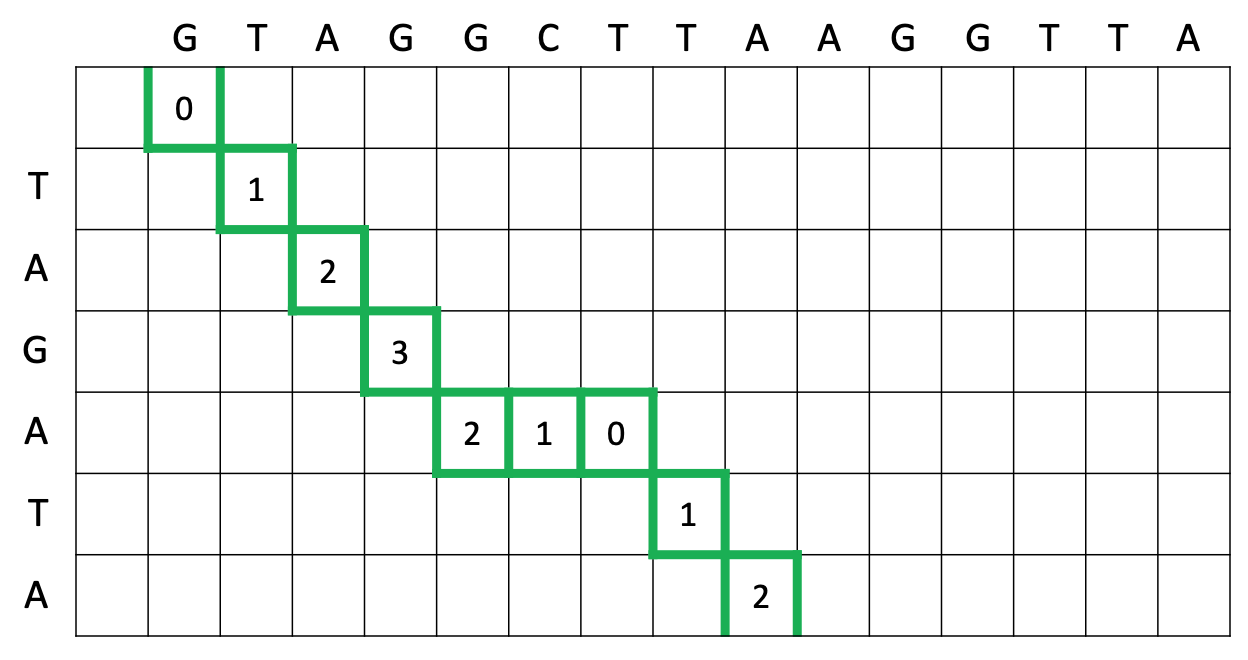
\includegraphics[scale=0.7]{2c_blank.png}
\end{center}

Give the fitting alignment corresponding to the highlighted path. [5 points]

\vspace{.5cm}

\fbox{\parbox{\linewidth}{

Corresponding alignment:
\begin{center}
\begin{tabular}{|p{.5cm}|p{.5cm}|p{.5cm}|p{.5cm}|p{.5cm}|p{.5cm}|p{.5cm}|p{.5cm}|p{.5cm}|p{.5cm}|p{.5cm}|p{.5cm}|p{.5cm}|p{.5cm}|p{.5cm}|p{.5cm}|p{.5cm}|}
\hline
\textcolor{gray}{-}   &\textcolor{red}T  &\textcolor{red}A  &\textcolor{red}G  &\textcolor{red}A  &\textcolor{red}-  &\textcolor{red}- &\textcolor{red}T  &\textcolor{red}A  &\textcolor{gray}{-}  &\textcolor{gray}{-}  &\textcolor{gray}{-}  &\textcolor{gray}{-}  &\textcolor{gray}{-}  &\textcolor{gray}{-}\\
\hline
\textcolor{gray}{G}   &\textcolor{red}T  &\textcolor{red}A  &\textcolor{red}G  &\textcolor{red}G  &\textcolor{red}C  &\textcolor{red}T &\textcolor{red}T  &\textcolor{red}A  &\textcolor{gray}{A} &\textcolor{gray}{G} &\textcolor{gray}{G}  &\textcolor{gray}{T}  &\textcolor{gray}{T} &\textcolor{gray}{A} \\
\hline
\end{tabular}
\end{center}
}}

\clearpage

\item[d.] Consider the following local alignment (grayed out entries are not part of the alignment). 
That is, an alignment of a substring of $\mathbf{v}$ and a substring of $\mathbf{w}$ with maximum global alignment score. 




% Local alignment is the second of the two fundamental alignment algorithms. In local alignment, the initial row and column of the dynamic programming table are initialized with zeroes. The score for a cell is the maximum of four scores (calculated according to the scoring matrix): the insertion, deletion, and match/mismatch scores, as well as the constant 0. The traceback starts at the largest value in the dynamic programming matrix and ends at the first 0 encountered.



\begin{center}
\begin{tabular}{ c | c c c c c c c c c c c c c c c } 
$\mathbf{v}$ & \textcolor{gray}{-} & \textcolor{red}{T} & \textcolor{red}{A} & \textcolor{red}{G}	&\textcolor{gray}{-}&	\textcolor{gray}{-}&	\textcolor{gray}{-} &	\textcolor{gray}{-} &	\textcolor{gray}{-} & \textcolor{gray}{-}	& \textcolor{gray}{-} &	\textcolor{gray}{-} &	\textcolor{gray}{-} &	\textcolor{gray}{-} &	\textcolor{gray}{-}\\
$\mathbf{w}$ & \textcolor{gray}{G} & \textcolor{red}{T} & \textcolor{red}{A} & \textcolor{red}{G} & \textcolor{gray}{G} & \textcolor{gray}{C} & \textcolor{gray}{T} & \textcolor{gray}{T} & \textcolor{gray}{A} & \textcolor{gray}{A} &	\textcolor{gray}{G} &	\textcolor{gray}{G} &	\textcolor{gray}{T} &	\textcolor{gray}{T} &	\textcolor{gray}{A}\\
\end{tabular}
\end{center}

Give the score for this local alignment and fill out the dynamic programming table with the corresponding backtrace (i.e. highlight the corresponding path through this table and fill in cells on path with alignment scores). [5 points]

\vspace{.5cm}

\fbox{\parbox{\linewidth}{


\vspace{.5cm}
\begin{center}
\scalebox{1.15}{
\hspace{-.3cm}
\begin{tabular}{|c|c|c|c|c|c|c|c|c|c|c|c|c|c|c|c|c|}
\hline
  &- &G  &T  &A  &G  & G & C & T &T  &A  & A  & G  & G  & T  & T  & A\\ \hline
- &0 &\cellcolor{red!25}0  &0  &0  &0  &0  &0  &0  &0  &0  &0   &0   &0   &0   &0   &0 \\ \hline
T &0 &0  &\cellcolor{red!25}1  &0  &0  &0  &0  &1  &1  &0  &0   &0   &0   &1  &1    &0 \\ \hline
A &0 &0  &0  &\cellcolor{red!25}2  &0  &0  &0  &0  &0  &2  &1   &0   &0   &0  &0    &2\\ \hline
G &0 &1  &0  &0  &\cellcolor{red!25}3  &1  &0  &0  &0  &1  &0   &2   &1   &0  &0    &1\\ \hline
A &0 &0  &0  &1  &0  &0  &0  &0  &0  &0  &1   &1   &1   &0   &0   &0 \\ \hline
T &0 &0  &1  &0  &0  &0  &0  &1  &1  &0  &0   &0   &0   &1   &1   &0 \\ \hline
A &0 &0  &0  &2  &0  &0  &0  &0  &0  &2  &1   &0   &0   &0   &0   &2  \\ \hline
\end{tabular}}
\end{center}
\vspace{.5cm}


Alignment score:  \underline{ \quad   3   \quad \quad   }
}}
\end{enumerate}


\clearpage


\item[3.] \textbf{Linear Space Alignment} [10 points]

Consider two sequences $\mathbf{v} = \mathrm{CT}$ and $\mathbf{w} = \mathrm{GCAT}$ of length $m = |\mathbf{v}| = 2$ and $n = |\mathbf{w}| = 4$, respectively.
In this exercise, we will compute an optimal global alignment of the two sequences using the Hirschberg algorithm.
We will use a score of +1 for a match, -1 for a mismatch, and -1 for a insertion/deletion (i.e.\ a gap penalty of 1).

\begin{enumerate}
  \item[a.] The initial call is \textsc{Hirschberg}($0,0,m=2,n=4$). We need to identify the middle vertex $(i^*,n/2=2)$. Fill out the following table for this initial call and indicate $i^*$. [2 points]
\\[.5em]
\fbox{\parbox{\linewidth}{


\begin{center}
\begin{tabular}{|c|c|c|c|}
\hline
$i$ & $\mathrm{prefix}(i)$ & $\mathrm{suffix}(i)$ & $\mathrm{wt}(i)$\\
\hline
0 &-2 &0 &-2\\
\hline
1 &0 &0 &0\\
\hline
2 &-1 &-2 &-3\\
\hline
\end{tabular}
\end{center}

}}

\item[b.] What are the two recursive calls that are made in this initial invocation \textsc{Hirschberg}($0,0,m,n$)? [1 point]
\\[.5em]
\fbox{\parbox{\linewidth}{


\begin{center}
  \textsc{Hirschberg}($\  0, \qquad 0\ ,\qquad 1, \qquad  2\qquad$) and \\\textsc{Hirschberg}($\ 1, \qquad 2, \qquad 2,\qquad 4\qquad$)
\end{center}

}}

\item[c.] Give the recursion tree, where each vertex corresponds to an invocation of \textsc{Hirschberg}.
See Lecture 1 for an example of a recursion tree. 
Label each vertex of this tree by the used arguments $(i,j,i',j')$. 
In addition, label each \emph{internal} vertex by the value of $i^*$, $\mathrm{prefix}(i^*)$ and $\mathrm{suffix}(i^*)$. [5 points]
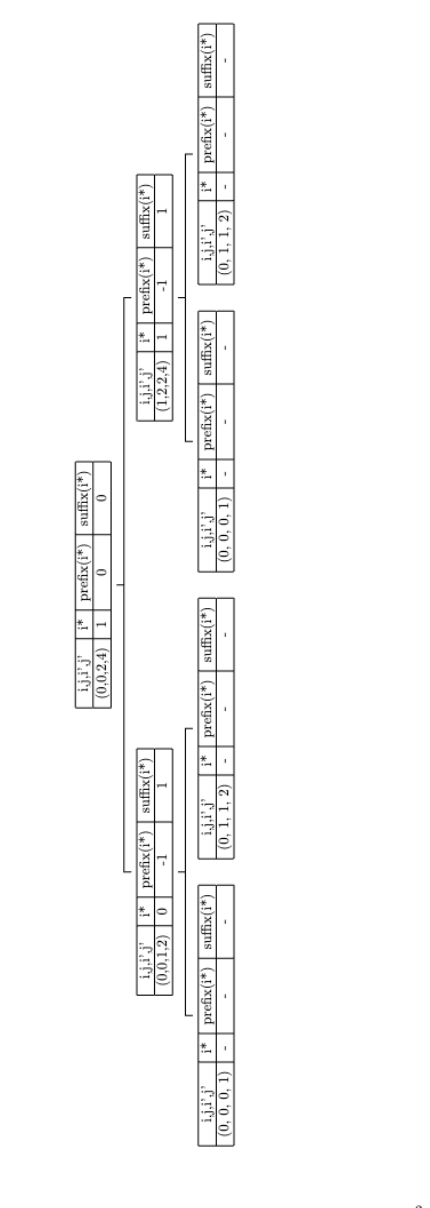
\includegraphics[scale=0.8, angle =-90]{RecursionTree.png}








%\\[.5em]
\clearpage
\item[d.] Indicate the reported vertices in the table and give the final alignment. [2 points]
\\[.5em]
\fbox{\parbox{\linewidth}{
Reported vertices (`X'):

\begin{center}
\begin{tabular}{|c|c|c|c|c|c|}
\hline
& 0 & G & C & A & T\\
\hline
0 & X &X & & & \\
\hline
C & & &X &X & \\
\hline
T & & & & & X \\
\hline
\end{tabular}
\end{center}

Final alignment:

\begin{center}
\begin{tabular}{|p{.5cm}|p{.5cm}|p{.5cm}|p{.5cm}|p{.5cm}|p{.5cm}|}
\hline
 -  &C  &-  &T   \\
\hline
 G  &C  &A &T   \\
\hline
\end{tabular}
\end{center}

}}

\end{enumerate}

\clearpage

\item[4.] \textbf{Banded Alignment} [5 points]

Global pairwise sequence alignment of two sequences of length $m$ and $n$ takes $O(mn)$ time using dynamic programming.
This corresponds to quadratic time.
In this question, we consider banded alignment, which was introduced in Lecture~5. Briefly, the idea is to restrict alignments, which are paths from $(0,0)$ to $(m,n)$, to only occur in a band of width $k$ around the diagonal. Modify the recurrence of global sequence alignment to achieve this change. Assume $m=n$ and use 0-based indexing, i.e.\ with $k=0$ the allowed region consists of only the diagonal, $k=1$ has an allowed region of length $3$, etc. [5 points]
\\[.5em]
\fbox{\parbox{\linewidth}{

\vspace{.8cm}
a  coordinate will be present in the band only if it satisfies following condition\\
$|i-j|$=k \\

The recurrence can be calculated as :-\\
\begin{equation*}
s[i,j] = \max
\begin{cases}
  0, & \mbox{if i=0, j=0,}\\
  s[i-1,j] + \delta(v_i, -), & \mbox{if j $\le$ i+k }\\
  s[i,j-1] + \delta(-, w_j), & \mbox{if j $\ge$ i-k }\\
  s[i-1,j-1] + \delta(v_i, w_j), & \mbox{otherwise }\\
\end{cases}
\end{equation*}
\vspace{.8cm}

}}
\end{enumerate}
% \fi

\clearpage

\begin{enumerate}
\item[5.] \textbf{BLOSUM} [10 points]

Consider the following three blocks on the alphabet $\Sigma = \{A,B,C,D\}$.

\begin{verbatim}
ABCDA         BBC       AAAA
ABCDA         BBC       DBBB
BBCDA         BCC       BAAA
AACDA         CBC       ADBA
CBADA         BBD
AACAA
\end{verbatim}

Using $L=0$, such that the above three blocks are not pruned down, compute the BLOSUM0 scoring matrix. Use $\lambda = 0.5$, the natural logarithm and round up to the nearest integer (i.e.\ take the ceiling). \textbf{Give $q_x$ and $p_{x,y}$ for each $x,y \in \Sigma$. Clearly indicate the denominator used for computing these two quantities.}

\fbox{\parbox{\linewidth}{
$q_{A}$= 23/61 = 0.377 \\
$q_{B}$= 18/61 = 0.295\\
$q_{C}$= 12/61 = 0.196\\
$q_{D}$=8/61 =0.131\\
\\
$q_{A, A}$= 22/129 = 0.170\\
$q_{A, B}$= 23/129 =0.178\\
$q_{A, C}$= 9/129 = 0.069\\
$q_{A, D}$= 9/129 = 0.069\\
$q_{B, B}$= 19/129 =0.147\\
$q_{B, C}$= 9/129 = 0.069\\
$q_{B, D}$= 2/129 = 0.016\\
$q_{C, C}$= 16/129 = 0.124 \\
$q_{C, D}$= 4/129 = 0.031 \\
$q_{D, D}$= 10/129 = 0.077 \\

\[ s(A, B) = \frac{1}{\lambda} \ln \frac{p_{A}p_{B}}{q_{A,B}}\]
\\
\bigskip
The BLOSUM scoring Matrix is as follows \\
\begin{center}
\begin{tabular} {c c c c c}

A &1 &   &  & \\
B &1 &2 & &  \\
C &0 &1 &3 &  \\
D &1 &-1 &1 &4 \\
 &A &B &C &D

\end{tabular}
\end{center}

 
\vspace{1cm}.

}}
\end{enumerate}

\clearpage
\begin{enumerate}
\item[6.] \textbf{Bonus: Total Number of Global Alignments} [6~points]

In this bonus question, we are going to determine the total number of \emph{global alignments} that exist given two strings $\mathbf{v} \in \Sigma^m$ and $\mathbf{w} \in \Sigma^n$. 
We will assume without loss of generality that $m \le n$.
Recall the matrix representation of an alignment. 
This is a $2 \times k$ matrix where $k \in \{\max\{m,n\},\ldots,m+n\}$ such that there is no column with two gaps.
Thus, the number $k$ of columns varies from $\max\{m,n\}$ to $m+n$.

\begin{itemize}
\item[a.] Explain why, in general (i.e.\ no prior knowledge on how $m$ and $n$ are related), the number $k$ of columns varies from $\max\{m,n\}$ to $m+n$. [1 point]




\fbox{\parbox{\linewidth}{
\vspace{1em}
Since alignment is way to convert one sequence to another, it needs minimum number of spaces to accommodate the  sequence of larger length, which is given by \textbf{max$\{ $m,n$\}$}.\\
Also we say that there shouldn't be any column with two gaps, and in the worst case, when no letters in v and w match,  we need to delete all elements of sequence v and  insert all letters of sequence w, which will need a space of m+n letters (n gaps in row 1 corresponding to n inserts and m gaps in row 2 corresponding to n deletes). Hence \textbf{maximum} number of columns required will be \textbf{m+n}\\
Thus, the number k of columns varies from \textbf{max$\{ $m,n$\}$} to \textbf{m+n}

.\vspace{1em}

}}

\item[b.]  
Explain why $k \in \{n,\ldots,m+n\}$ for the case where $m \le n$. [1 point]

\fbox{\parbox{\linewidth}{
\vspace{1em}
Using the above explanation in 6b , we know that the number k of columns varies from \textbf{max$\{ $m,n$\}$} to \textbf{m+n}. \\
If m $\le$ n , then \textbf{max $\{ $ m,n $ \}$ } = n .
\\Hence in that case the number of k of columns varies from \textbf{n} to \textbf{m+n} , that is k \in $\{ $ n,  ..., m+n $\} $
.\vspace{1em}

}}


\item[c.] Suppose that the alignment has length $k \ge n$. In how many different ways can we insert $k - n$ gaps in the second sequence $\mathbf{w}$, yielding gapped sequence $\mathbf{w}'$? [1~point]

\emph{Hint:} Observe that $\mathbf{w}'$ has length $k$.

\fbox{\parbox{\linewidth}{

kC (k-n) = kC n
.\vspace{5em}

}}

\item[d.] Let $\mathbf{w}'$ be a gapped sequence of length $k \in \{n,\ldots,m+n\}$ such that removing the gaps yields the original sequence $\mathbf{w}$. 
In how many ways can we insert gaps in $\mathbf{v}$ to obtain an alignment with $\mathbf{w}'$ of length $k$?  [1~point]

\emph{Hint:} Recall that an alignment does not contain columns with two gaps. In how many different ways can we insert gaps in $\mathbf{v}$ subject to this condition?

\fbox{\parbox{\linewidth}{

.\vspace{12em}

}}

\item[e.] How many alignments of $\mathbf{v}$ and $\mathbf{w}$ are there of a given length $k \in \{n, \ldots, m+n\}$? How many alignments are there of any length? [1~point]

\emph{Hint:} Combine your answers to the previous two questions.

\fbox{\parbox{\linewidth}{

Number of alignments of of any length 
\[
    \binom{m+n}{n} = \frac{(m+n)!}{m!n!}
\]


}}


\item[f.] Give an example of a scoring function $\delta : (\Sigma \cup \{-\}) \times (\Sigma \cup \{-\}) \rightarrow \mathbb{R}$ such that the number of optimal global alignments equals your answer to the previous question. [1~point]

\emph{Hint:} Think of a border case.

\fbox{\parbox{\linewidth}{

.\vspace{8em}

}}

\end{itemize}
\end{enumerate}

\end{document}
